\documentclass[11pt]{article}

% Language setting
% Replace `english' with e.g. `spanish' to change the document language
\usepackage[english]{babel}
\usepackage{biblatex}
% Set page size and margins
% Replace `letterpaper' with `a4paper' for UK/EU standard size
\usepackage[letterpaper,top=2cm,bottom=2cm,left=3cm,right=3cm,marginparwidth=1.75cm]{geometry}

% Useful packages
\usepackage{amsmath}
\usepackage{graphicx}
\usepackage[colorlinks=true, allcolors=blue]{hyperref}
\usepackage{titling}
\bibliography{Final_Report_Ref.bib}
\renewcommand\maketitlehooka{\null\mbox{}\vfill}
\renewcommand\maketitlehookd{\vfill\null}

\title{%
  Identifying Man's Best Friend \\
  \; \\
  \large Final Report}

\author{Edward Wang}
\date{Spring 2024}

\begin{document}

\begin{titlingpage}
\maketitle
\end{titlingpage}

\newpage

\tableofcontents

\newpage

\section{Problem Statement}

For centuries, dogs have stood as steadfast companions to humans, earning the endearing title of "man's best friend." This remarkable bond traces back thousands of years. Dogs were domesticated more than 10,000 years ago in Europe \cite{dog1}, with earlier ties in other regions of the world. Initially serving as hunting partners, guardians, and eventually cherished members of the family, dogs have evolved and adapted to various roles and environments. From the loyal sled dogs of the Arctic to the quite literal definition of role by acting in various movies, their versatility and loyalty made them beloved across diverse cultures worldwide. 

Today, dogs are the most popular pet in the U.S., with 65.1 million households  proudly owning a dog \cite{forbes}. That's 1 in every 2 households! The American Kennel Club (AKC) recognizes 200 distinct breeds \cite{akc}, some of which bear striking resemblances to each other despite possessing notably different temperaments. As depicted in Figure \ref{fig:husky}, the Siberian Husky is well known for its stubbornness and independent nature     \cite{akc_husky}, while the Alaskan Malamute, nearly twice its weight, tends to exhibit characteristics more akin to those of a watchdog \cite{akc_mal}. 

\begin{figure}[h]
\centering
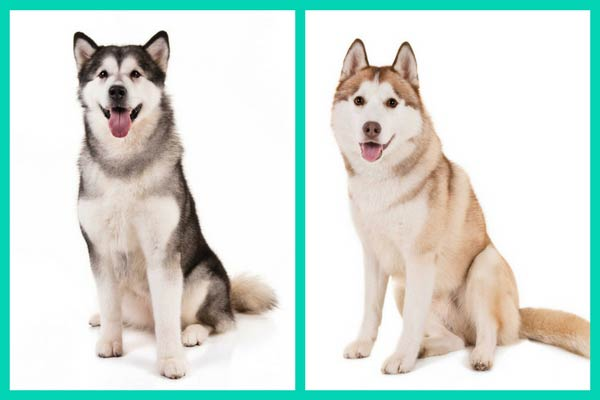
\includegraphics[width=0.25\linewidth]{malamutehusky.jpg}
\caption{\label{fig:husky}Alaskan Malamute (Left) and Siberian Husky (Right)}
\end{figure}

There are various other breeds that are very similar. For example, the Border Collie and Australian Shepherd is another close looking pair. \textbf{The objective is to explore and develop a Neural Network capable of accurately identifying various breeds of dogs.}

% \newpage

\section{Data Collection}

\subsection{Data Source}

The data source for this project is the Stanford Dogs Dataset \cite{data_source}, which contains images of 120 breeds of dogs from around the world. This dataset is part of the larger ImageNet dataset with annotations and labels. The Stanford Dogs Dataset contains colored images of dogs in various poses and locations. Within Figure \ref{fig:golden}, the Golden Retriever breed is depicted in three distinct scenarios: engaging in play with a ball, enjoying a swim, and receiving affection from their owner. These varied poses offer real-world examples of where one might encounter their four-legged companion. These images serve to diversify the model's learning experience beyond merely recognizing dog breeds from textbooks.

\begin{figure}[htb]
\centering
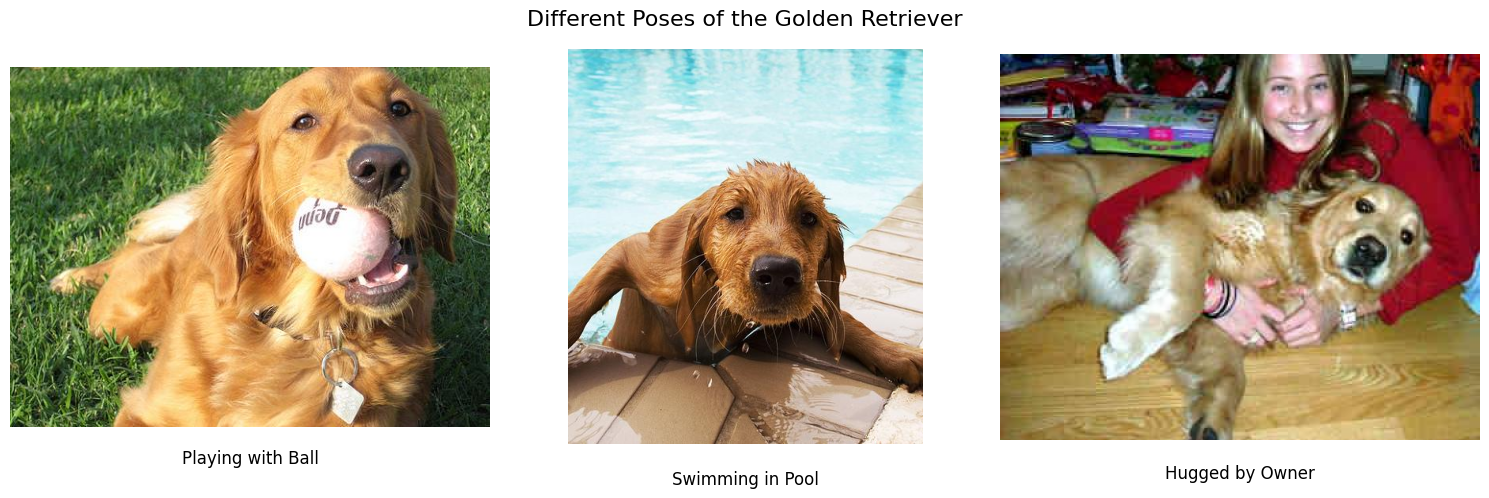
\includegraphics[width=1\columnwidth]{golden_retriever_poses.png}
\caption{\label{fig:golden}Golden Retriever in Different Poses}
\end{figure}

\newpage

There are seven recognized groups of dogs by the AKC, each categorized based on their physical attributes and personality traits: Working, Herding, Hound, Sporting, Non-Sporting, Terrier, and Toy. It's worth noting that the AKC website also includes two additional groups ("miscellaneous-class" and "foundation-stock-service"). However these are excluded due to limited data availability.

Due to a lack of an existing mapping of dog groups and breeds, one was created by scraping data from the AKC website. Regex and fuzzy matching were leveraged to sort the 120 dog breeds into their respective groups based on this data. We can see in Figure \ref{fig:group_counts} the unique number of dog breeds in each of different dog groups. We can see the lack of dog breeds that fall into the "miscellaneous-class" and the "foundation-stock-service" groups. It is important to note that breeds such as the Dingo, Dihole, and African Hunting Dog, which don't fit the typical archetype of a traditional family pet, have been excluded from this analysis. 

\begin{figure}[h]
\centering
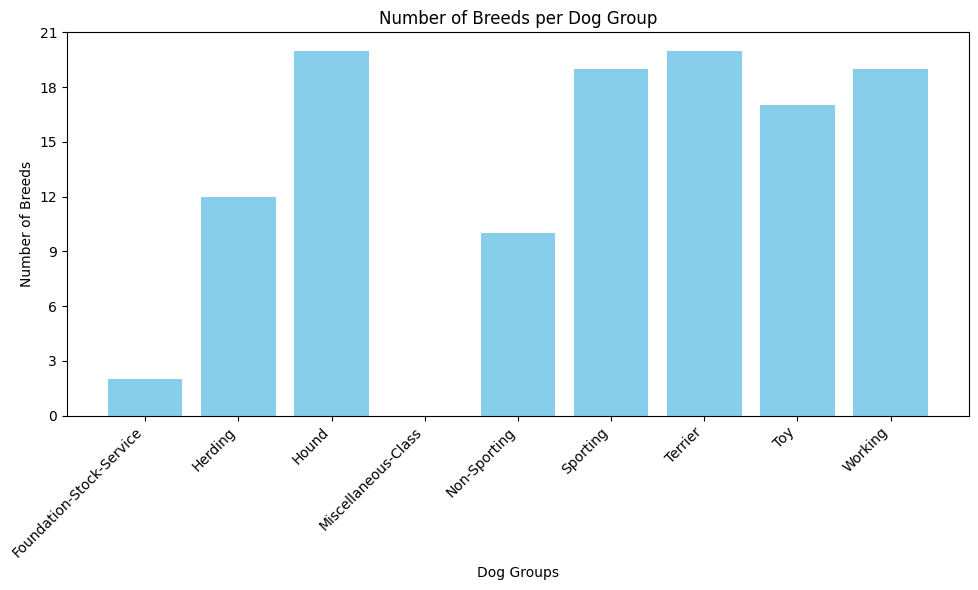
\includegraphics[width=1\columnwidth]{groups_breed_counts.png}
\caption{\label{fig:group_counts}Number of Distinct Breeds per Group}
\end{figure}

\newpage

\subsection{Data Preprocessing}

Opting for the Working group out of the seven distinct groups was a strategic decision. Focusing on a single group streamlines the project's manageability in terms of training times and individual contributions. Within the Working group, there are 19 distinct breeds encompassing a total of 3,295 images. Figure \ref{fig:image_counts} illustrates a relatively even distribution of images across the various breeds. This balance minimizes the risk of the model overfitting to any particular breed, eliminating the need for downsampling or upsampling techniques.

\begin{figure}[h]
\centering
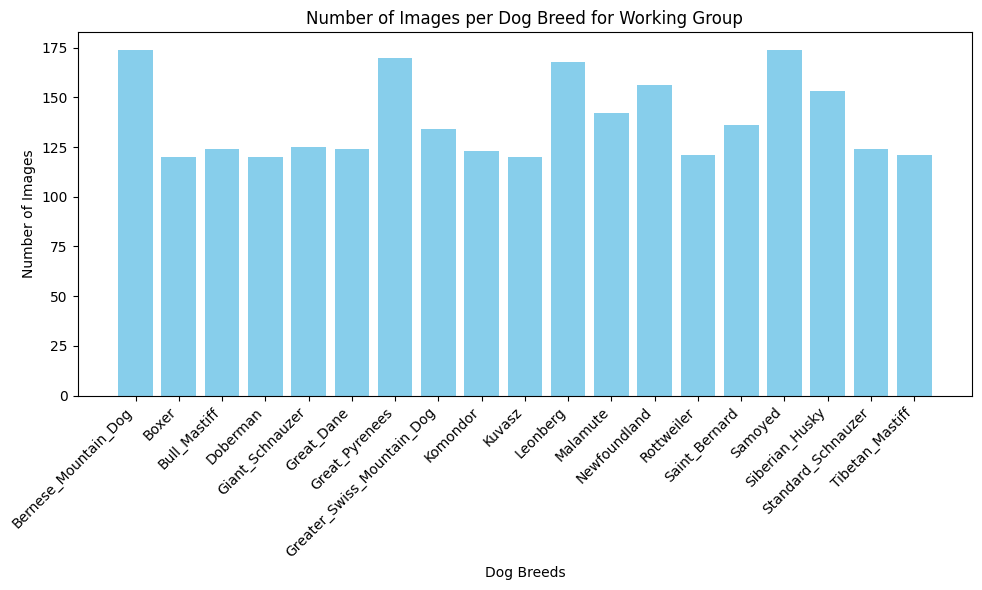
\includegraphics[width=1\columnwidth]{working_image_counts.png}
\caption{\label{fig:image_counts}Number of Images per Dog Breed}
\end{figure}

To ensure uniformity in the dataset, all images from the Stanford Dog Dataset are resized to a standardized resolution. Opting for a resolution of 224x224 pixels strikes a balance between computational efficiency and image clarity. This resizing process normalizes the images to dimensions of 224x224x3, where 3 denotes the RGB color channels.

Following the standard practice, dataset is partitioned into training and testing sets using an 80/20 split. Additionally, the training set is divided into an 80/20 split for training and validation purposes during the model training phase. This provides us 2,111 images for training across 19 classes, 518 images for validation, and 666 images for testing. The \texttt{ImageDataGenerator} function from Keras generates a single image each time it's called. Pairing \texttt{ImageDataGenerator} with \texttt{flow\_from\_directory} function allows direct to the images from the respective training and testing file directories.  

\subsection{Image Augmentation}

Given the relatively small number of training images available for each breed, even though most have more than 100 images, the dataset remains limited for effective image classification. Therefore, leveraging image augmentation becomes essential to artificially expand the dataset and enhance the model's ability to generalize effectively across diverse scenarios.

Image augmentation involves applying diverse transformations to existing images, including rotation, flipping, and cropping, to artificially increase the dataset's size. For instance, the shift range adjustment relocates the images, placing the dog in different positions within the frame. Similarly, sheer range distorts the image along specific axes, while brightness variations simulate varying lighting conditions. These transformations are summarized in Table \ref{tab:image_aug_pram} below.

\begin{table}[h]
    \centering
    \caption{Parameters for Augmented Dog images}
    \label{tab:image_aug_pram}
    \begin{tabular}{|c|c|}
    \hline
    \textbf{Transformation} & \textbf{Value} \\
    \hline
    Rotation range & 15 \\
    Width shift range & 0.1 \\
    Height shift range & 0.1 \\
    Shear range & 0.01 \\
    Zoom range & [0.9, 1.25] \\
    Horizontal flip & True \\
    Fill mode & nearest \\
    Brightness range & [0.5, 1.5] \\
    \hline
    \end{tabular}
\end{table}

In Figure \ref{fig:image_aug} below, we can observe examples of these transformations, with the original image depicted in the middle. Notice how the image is shifted to different positions and horizontally flipped in some instances. These adjustments effectively create variations of the original image, enabling the model to perceive them as distinct inputs.

\begin{figure}[!h]
\centering
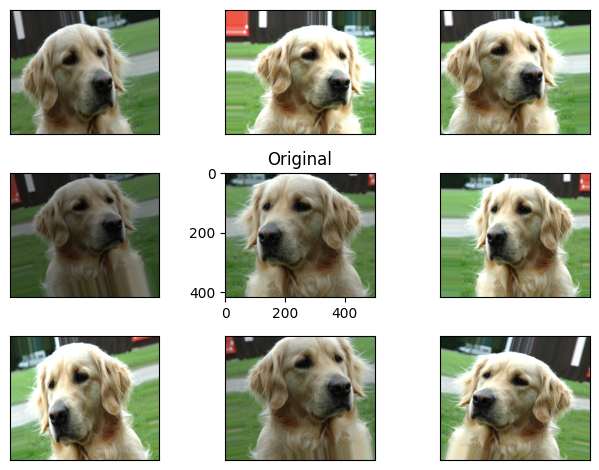
\includegraphics[width=1\columnwidth]{image_augmentation_sample.png}
\caption{\label{fig:image_aug}Image Augmentation}
\end{figure}

% \subsection{Data Flowchart}  


\section{Methodology}

\subsection{Introduction}

The objective is to identify the various breeds of dogs, so the best model would be a image classification model. Specifically, for image classification the Convolutional Neural Network (CNN) is the best. CNN is a Deep Learning Neural Network that can take in an input image, assign the weights and biases, and produce a final prediction\cite{cnn}.  

In contrast to traditional Neural Networks, Convolutional Neural Networks (CNNs) are characterized by their convolutional layers, which play a crucial role in the feature extraction process. These layers contain filters, or kernels, that capture important features and patterns present in the input image, such as edges, textures, and shapes. For instance, in a scenario distinguishing between a slice of pie and a whole pie, a CNN would learn to differentiate the unique triangular shape of the slice from the round circle of the whole pie. Similarly, in the context of the dog dataset, CNNs would identify features like fur length, snout length, or the shape of the head and tail.

One process to speed up training and improve accuracy is to leverage transfer learning. Transfer learning is the process of using the pre-trained CNN as a starting point and fine-tuning it on the new dataset. Essentially, this fine-tuning process is only training the last few layers of the CNN on the new dataset. Some of the major pre-trained CNNs on large image datasets are ResNet, VGG16, Inception-v3, and MobileNet.

\subsection{DenseNet121}

In this project, DenseNet is used as the pre-trained CNN architecture, with a specific focus on DenseNet121. DenseNet, introduced in 2016, represents an advancement over the ResNet model developed in 2014\cite{timeline}. 

ResNet introduced the concept of residual connections. In a residual block, the input to a layer is added to the output of the layer, allowing for easier training of deep networks by mitigating the vanishing gradient problem. Densenet further improves this concept by introducing dense connections. Specifically, DenseNets concatenates the output feature maps of the layer with the incoming feature maps instead of summing them like in ResNet. We can see a detailed architecture of DenseNet in Figure \ref{fig:densenet_arch} from Densely Connected Convolutional Networks \cite{densenet_arc}

\begin{figure}[h]
\centering
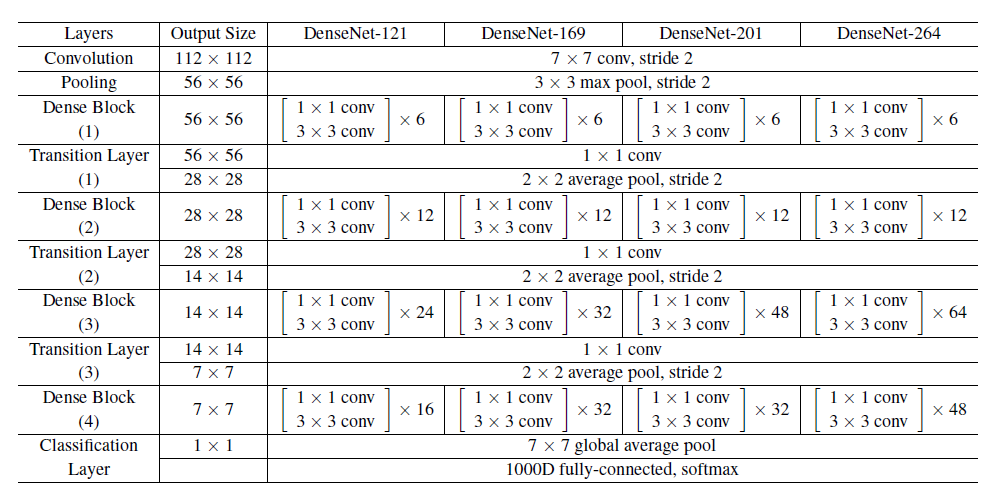
\includegraphics[width=0.74\columnwidth]{densenet_arch.png}
\caption{\label{fig:densenet_arch}Sizes of Kernels for Various DenseNets \cite{densenet_arc} architectures on ImageNet}
\end{figure}

\pagebreak

\subsection{Model Architecture}

In the final trained model, in addition to the layers inherited from DenseNet121, supplementary layers are included, as illustrated in Figure \ref{fig:model_arch}. These additional layers start from the global average pooling, followed by three dense layers designed to reduce the output dimensions to 19, aligning with the number of classes. Additionally, dropout layers are introduced to randomly deactivate nodes which help prevent overfitting. In the final layer, a softmax function is employed to select the prediction with the highest probability as the final label.

\begin{figure}[h]
    \centering
    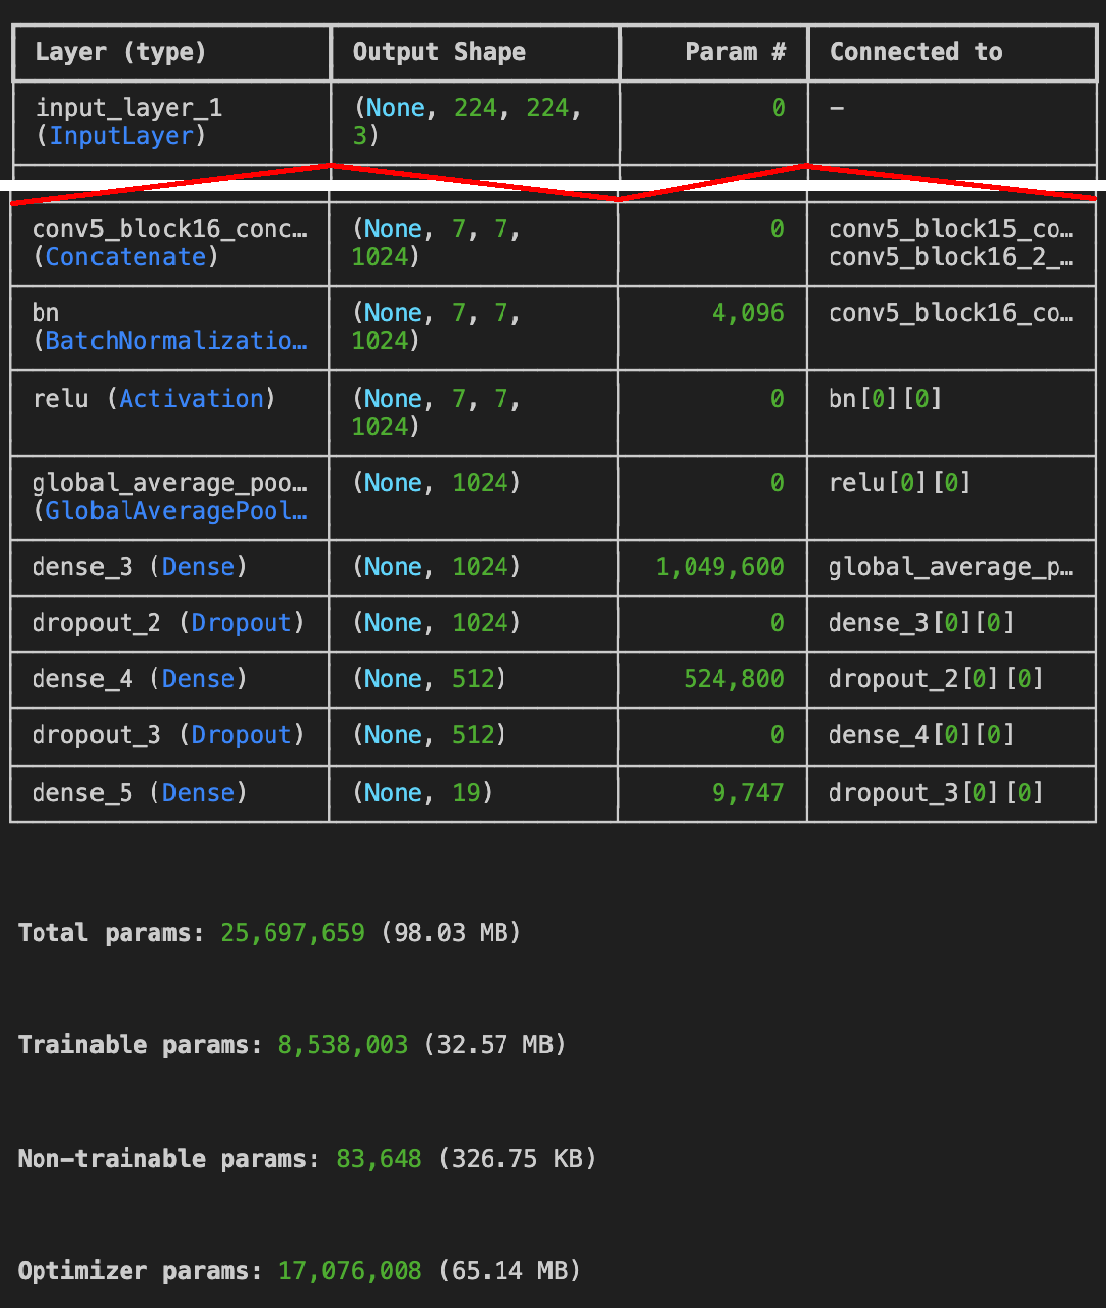
\includegraphics[width=0.5\linewidth]{model_arch.png}
    \caption{\label{fig:model_arch}Trained Model Architecture}
\end{figure}

We can see that DenseNet121 comprises a total of 25.7 million parameters. By unfreezing the last 20 layers, 8.5 million parameters become trainable. The supplementary layers contribute 1.5 million parameters out of the 8.5 million.

\subsection{Model Parameters}

In this model, a batch size of 32 is selected, striking a balance between computational efficiency and the model's generalization capacity. While a larger batch size could expedite convergence, it also heightens the risk of overfitting and demands more memory resources. Given that this model is trained on a laptop, opting for a smaller batch size is preferable.

During model training, besides utilizing image augmentation, additional regularization techniques are employed. One such method involves decreasing the learning rate when the validation accuracy plateaus. In this model, if there's no improvement in validation accuracy after 1 epoch, the learning rate is reduced by a factor of 0.2, followed by a cooldown period of 2 epochs.

Additionally, early stopping is utilized as another regularization technique. This strategy halts the training process prematurely if there's insignificant improvement in accuracy. The validation loss serves as the metric, with a threshold set at 5 epochs of no improvement.

Finally, the optimal model weights are saved for future reference reducing the need to retrain the model each time. This approach minimizes computational overhead and allows efficient model deployment for subsequent predictions.

\subsection{Model Training}


The final trained model achieved an accuracy of 0.67 and a validation accuracy of 0.69. Notably, the validation accuracy occasionally surpassed the training accuracy, potentially influenced by the dropout layers and the absence of shuffling during training. Moreover, the validation accuracy dropping to 0 at epoch 2 suggests potential issues in the model training process relative to the inputs. Further examination may be warranted in the future to address potential issues and refine the model's performance.

\begin{figure}[h]
    \centering
    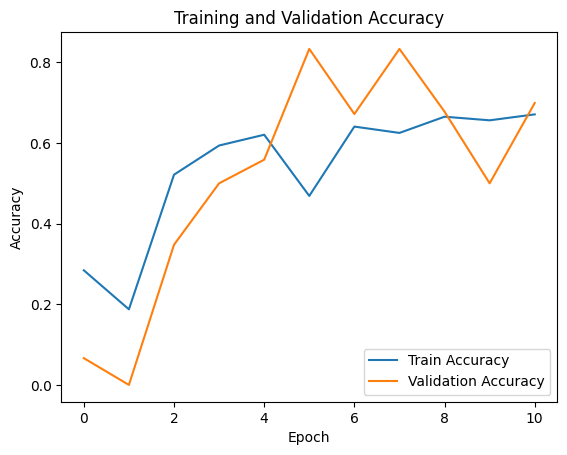
\includegraphics[width=0.5\linewidth]{model_accuracy.png}
    \caption{\label{fig:model_acc}Model Training Accuracy}
\end{figure}

\section{Model Evaluation}

\subsection{Testing Dataset}

The testing dataset comprises 666 images distributed evenly among the 19 classes. There's a relatively balanced representation of each class.

\begin{figure}[h]
    \centering
    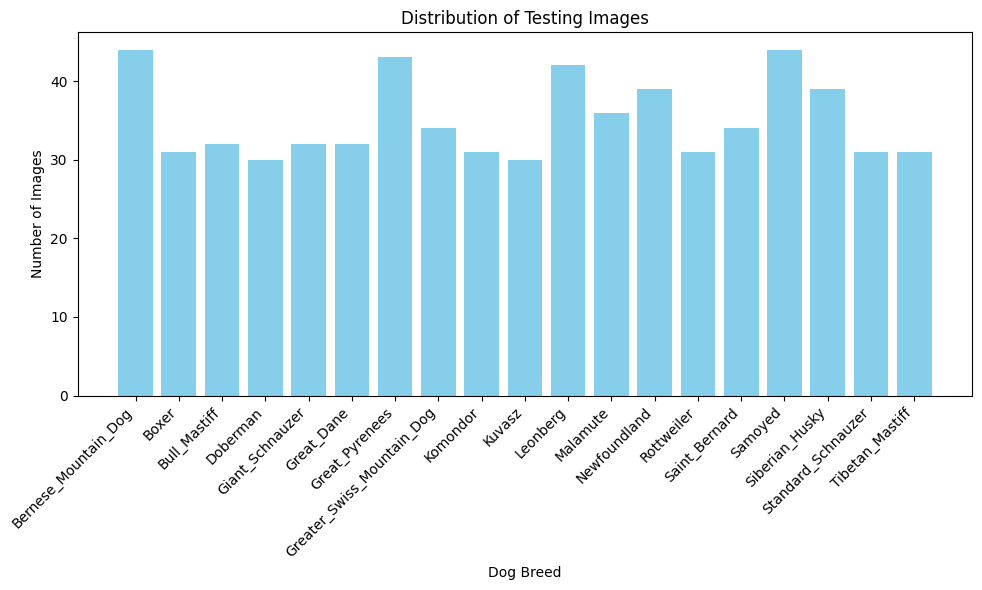
\includegraphics[width=0.5\linewidth]{testing_image_counts.png}
    \caption{\label{fig:testing_img}Number of Images in Testing Dataset }
\end{figure}

\newpage

\subsection{F1 Score}

The averaged F1 score is around 0.6366. Some of the worst performing breeds are Kuvasz, Greater Swiss Mountain Dog, and Boxer. We can see the rest of the F1 scores in Table \ref{tab:classification_report}. We will take a look at why later on in the report.     

Breeds such as the Great Swiss Mountain Dog and the Boxer exhibit high precision but low recall in the model's predictions. This indicates that the model is conservative in its predictions for these breeds, confidently identifying the few positive instances it predicts but missing a significant number of actual positive instances.

Conversely, breeds like the Samoyed and Bernese Mountain Dog demonstrate low precision but high recall. This suggests that the model identifies most of the actual positive instances but is susceptible to false positives, potentially due to misclassification or ambiguity in distinguishing features.


\begin{table}[htbp]
\centering
\caption{Classification Report}
\label{tab:classification_report}
\begin{tabular}{lcccc}
\hline
\textbf{Class}                 & \textbf{Precision} & \textbf{Recall} & \textbf{F1-score} & \textbf{Support} \\ \hline
Giant\_Schnauzer             & 0.54               & 0.59            & 0.57               & 32               \\
Standard\_Schnauzer          & 0.67               & 0.45            & 0.54               & 31               \\
Kuvasz                       & 0.40               & 0.20            & 0.27               & 30               \\
Komondor                     & 0.76               & 0.94            & 0.84               & 31               \\
Rottweiler                   & 0.88               & 0.48            & 0.62               & 31               \\
Doberman                     & 0.67               & 0.80            & 0.73               & 30               \\
Greater\_Swiss\_Mountain\_Dog & 0.83               & 0.29            & 0.43               & 34               \\
Bernese\_Mountain\_Dog       & 0.59               & 0.93            & 0.72               & 44               \\
Boxer                        & 0.90               & 0.29            & 0.44               & 31               \\
Bull\_Mastiff                & 0.70               & 0.88            & 0.78               & 32               \\
Tibetan\_Mastiff             & 0.83               & 0.61            & 0.70               & 31               \\
Great\_Dane                  & 0.58               & 0.66            & 0.62               & 32               \\
Saint\_Bernard               & 0.84               & 0.94            & 0.89               & 34               \\
Malamute                     & 0.56               & 0.64            & 0.60               & 36               \\
Siberian\_Husky              & 0.75               & 0.46            & 0.57               & 39               \\
Leonberg                     & 0.92               & 0.79            & 0.85               & 42               \\
Newfoundland                 & 0.58               & 0.79            & 0.67               & 39               \\
Great\_Pyrenees              & 0.50               & 0.51            & 0.51               & 43               \\
Samoyed                      & 0.53               & 0.93            & 0.68               & 44               \\ \hline
Accuracy                      &                    &                 & 0.65               & 666              \\
\textbf{Macro avg}            & 0.69               & 0.64            & 0.63               & 666              \\
\textbf{Weighted avg}         & 0.68               & 0.65            & 0.64               & 666              \\ \hline
\end{tabular}
\end{table}

\subsection{Confusion Matrix}

Figure \ref{fig:cm} sheds light on the model's challenges with certain breeds, revealing instances of confusion between similar breeds. For instance, the model struggles to differentiate between breeds such as Kuvasz and Great Pyrenees, both characterized by their large, white, fluffy appearance. Similar confusion arises between breeds like Giant Schnauzer and Standard Schnauzer, Rottweiler and Doberman, as well as Boxer and Bull Mastiff. Conversely, breeds with more distinct features, like the Newfoundland dog, are identified more accurately, as expected.

\begin{figure}[h]
    \centering
    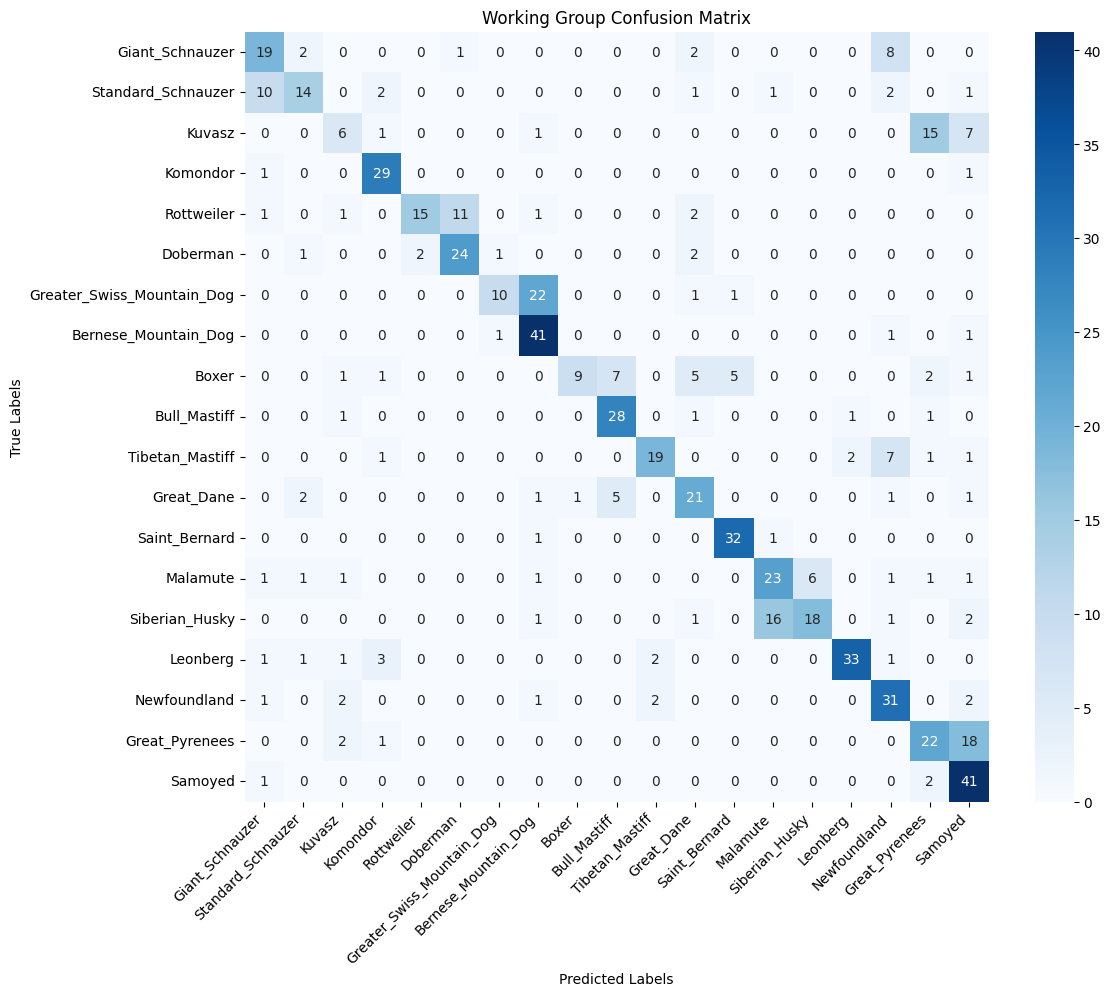
\includegraphics[width=1\linewidth]{confusion_matrix.png}
    \caption{\label{fig:cm}Confusion Matrix}
\end{figure}

\newpage

\subsection{Investigation}

By randomly selecting 16 images, the model achieved correct identifications for 10 of them. Particularly challenging were distinctions between Siberian Husky and Malamute, where the model struggled. Additionally, the model encountered difficulty in distinguishing Boxer breeds. Notably, the image of the Malamute lying on its side, predominantly white, could understandably lead to misidentifying as a Kuvasz. 


\begin{figure}[h]
    \centering
    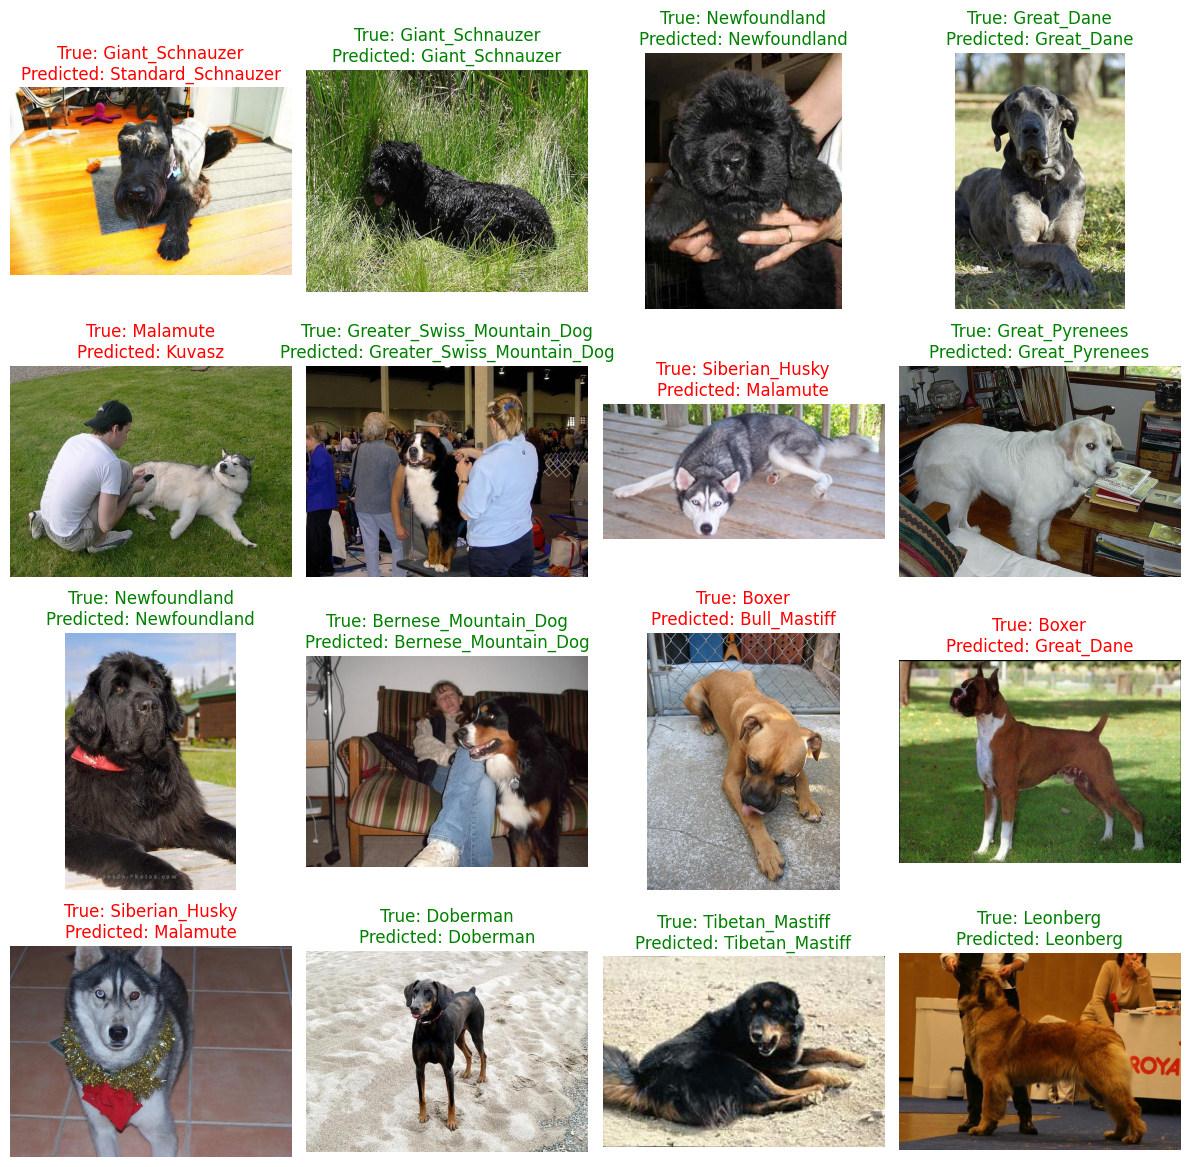
\includegraphics[width=1\linewidth]{random_classified.png}
    \caption{\label{fig:rnd_class}Randomly Selected True and Predicted Labels}
\end{figure}
\clearpage

Upon closer examination of the Schnauzer image, the perspective makes it challenging to accurately assess the size of the dog, a crucial factor in distinguishing between the standard and giant Schnauzer breeds. Initially, the Schnauzer may appear relatively small, but human observers can utilize contextual cues such as the octopus toy in the background and the rug to infer its actual size. However, a model lacks the same contextual understanding and may struggle to make accurate size differentiation.

\begin{figure}[h]
    \centering
    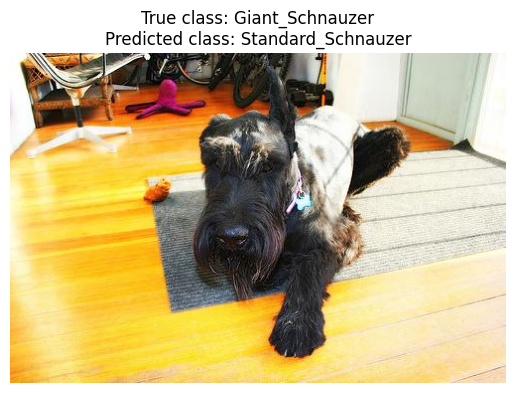
\includegraphics[width=1\linewidth]{schnauzer.png}
    \caption{\label{fig:schnauzer}Schnauzer Image}
\end{figure}

Furthermore, we observe two distinct images of an adorable puppy in Figure \ref{fig:puppies}, both labeled as Great Pyrenees. Despite their similarity, an individual unfamiliar with  the dog breed might struggle to distinguish between them. Consequently, the model assigns different predictions for each image. In both cases, the model's top two guesses are Samoyed and Great Pyrenees, each with around 30\% probability with Kuvasz following closely behind. 

The probability provides additional insight suggesting that the model's final prediction is relatively accurate. However, as indicated by the confusion matrix, the model struggles to make the final differentiation between various breeds. Unique breeds like Komondor poses no difficulty for the model as seen in Figure \ref{fig:komondor}.

\begin{figure}[h]
    \centering
    \begin{minipage}{0.45\textwidth}
        \centering
        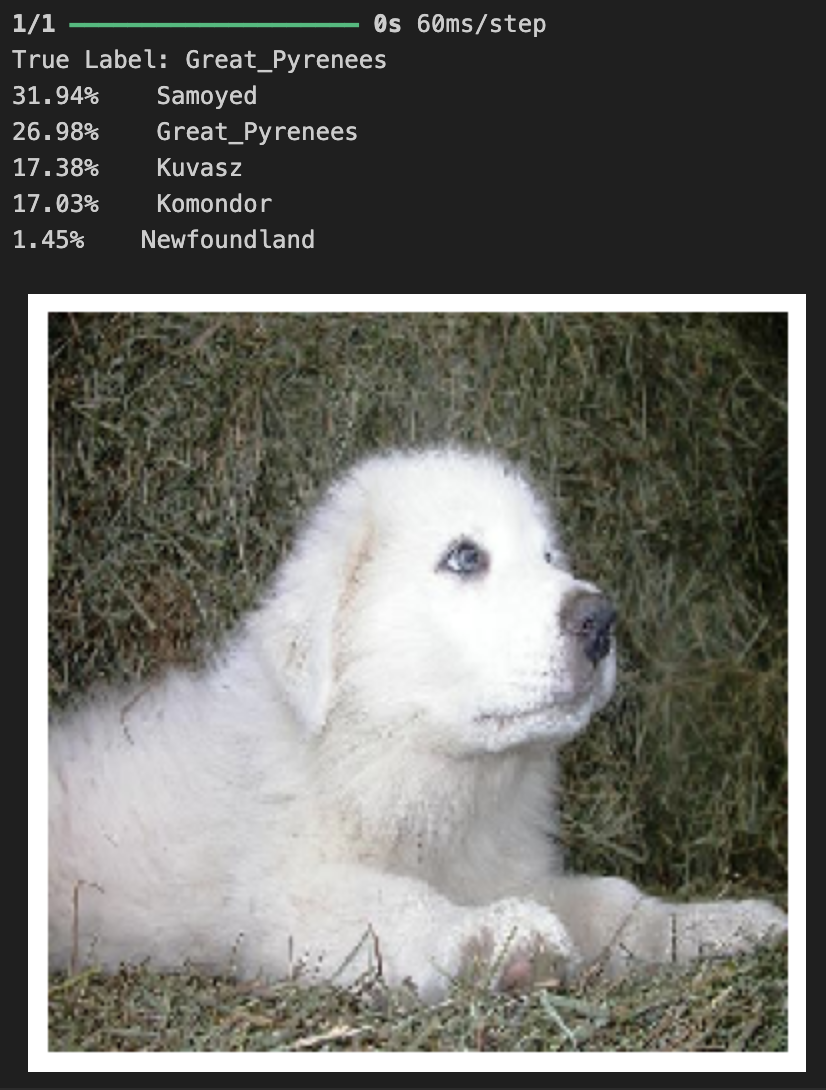
\includegraphics[width=0.9\textwidth]{puppy_1.png} % first figure itself
        \caption{Model Predicting Samoyed}
    \end{minipage}\hfill
    \begin{minipage}{0.45\textwidth}
        \centering
        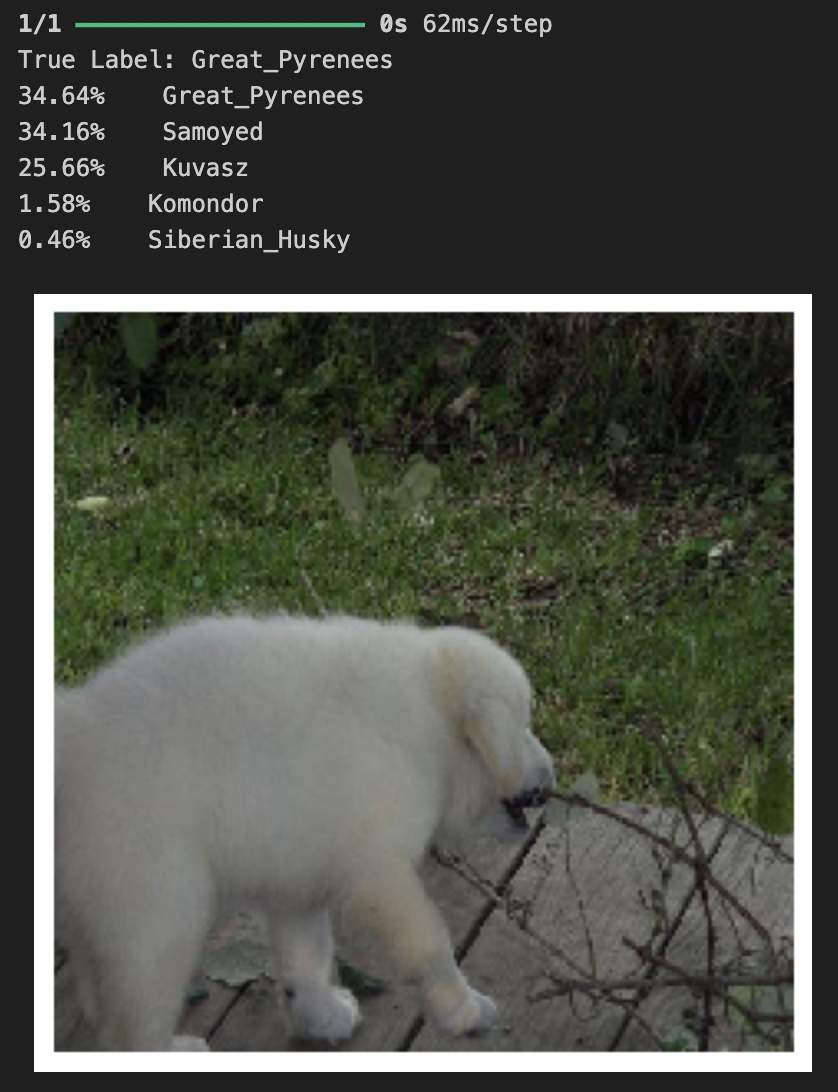
\includegraphics[width=0.9\textwidth]{puppy_2.png} % second figure itself
        \caption{Model Predicting Great Pyrenees}
    \end{minipage}
    \caption{\label{fig:puppies}Two Great Pyrenees Puppies}
\end{figure}

\begin{figure}[h]
    \centering
    \includegraphics[scale=0.5]{komondor.png}
    \caption{\label{fig:komondor}Komondor Image}
\end{figure}

\newpage
\clearpage
\section{Conclusion}

\subsection{Final Results}

The objective of exploring and developing a Neural Network capable of accurately identifying various breeds of dogs has been largely achieved. Through the utilization of the DenseNet121 architecture coupled with image augmentation techniques and regularization methods, a model was trained to classify 19 different breeds of dogs with a testing accuracy of around 67\%.

While the model demonstrates significant proficiency in identifying certain breeds, such as Komondor and Saint Bernard, it encounters challenges in distinguishing between breeds with similar characteristics, such as Kuvasz and Great Pyrenees. This is reflected in the confusion matrix and the F1 scores, indicating areas for potential improvement.

The investigation into misclassifications provided valuable insights into the model's decision-making process, highlighting instances where contextual understanding and nuanced features play crucial roles. Further refinement and fine-tuning of the model, potentially incorporating additional data and advanced techniques, could enhance its performance and address these challenges.

Overall, the Convolutional Neural Network represents a solid foundation for breed identification in dogs. It demonstrated promising accuracy and showcasing the potential of machine learning in dog breed classification. With continued development and refinement, it holds the potential to serve as a valuable tool in various application such as animal shelters. 

\subsection{Future Improvements}

There are several avenues for significant improvements to this model. Firstly, increasing the number of images per class would notably enhance its accuracy. With more diverse examples for each breed, the model could better grasp the subtle nuances unique to each, improving its ability to distinguish between similar breeds.

Additionally, revisiting the model architecture and fine-tuning hyperparameters such as the number of layers, batch size, and image augmentation techniques could yield significant gains. With access to better hardware, it would be feasible to experiment with multiple models simultaneously, enabling more comprehensive comparisons and optimizations.

Another promising approach would involve implementing an upstream model trained to classify breeds into broader dog groups initially. Subsequently, separate downstream models could be trained for each group, specializing in the classification of specific breeds within their respective categories. This hierarchical approach could streamline the classification process and potentially lead to more accurate results.

In conclusion, enhancing the model's accuracy can be achieved through increasing the training data, fine-tuning model architecture and hyperparameters, and implementing hierarchical classification approaches. 

\clearpage

\section{References} 
\printbibliography[heading=none]
% \bibliographystyle{plain}
% \bibliography{Final_Report_Ref}%writing the bibliography
% \addcontentsline{toc}{chapter}{References}%Including it as a chapter
\end{document}